\chapter{Configuration de la station}

\section{Création et installation de la distribution \textit{Raspbian}.}

Pour une \textit{RaspberryPi}, son disque dur est nulle autre qu'une carte Micro SD. C'est donc sur ce support que nous allons faire l'installation.

Pour réaliser cette étape, vous aurez besoin de :
\begin{itemize}
	\item d'une \textit{RaspberryPi}
	\item d'une carte micro SD de minimum 4Go
	\item du logiciel \href{etcher.io}{Etcher}
	\item de \href{https://sourceforge.net/projects/dexterindustriesraspbianflavor/}{\textit{Raspbian}}. En réalité il s'agit d'une version modifiée par la société Dexter Industries qui est spécialisé dans l'utilisation de \textit{RaspberryPi} pour la robotique.
	\item d'un adaptateur pour relier la micro SD à votre ordinateur.
\end{itemize}\\
Nous pouvons désormais commencer l'installation de l'OS sur notre \textit{RaspberryPi}

\begin{enumerate}
	\item Connecter la micro SD sur votre ordinateur.\\
	\item Lancer le logiciel \textit{Etcher}\\
	\begin{figure}[H]
	\begin{center}
		\makebox[\textwidth]{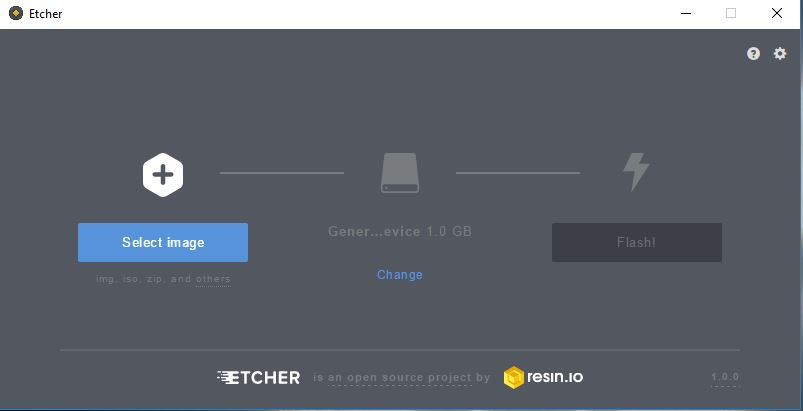
\includegraphics[width=.6\paperwidth]{images/etcher1.jpg}}
	\end{center}
		\caption{ \textit{Logiciel Etcher au lancement}}
	\end{figure}\\
	\item Cliquer sur \textit{"Select image"} à gauche puis sélectionner le fichier \textit{.zip} récupéré depuis le site \textit{SourceForce} dans les pré-requis.\\
	\item Vérifier que le périphérique qui est renseigné au centre est bien la micro SD. Dans le cas contraire cliquer sur \textit{"Change"}.\\
	\item Si les deux étapes précédentes sont OK, cliquer sur \textit{"Flash"}.\\
	\begin{figure}[H]
	\begin{center}
		\makebox[\textwidth]{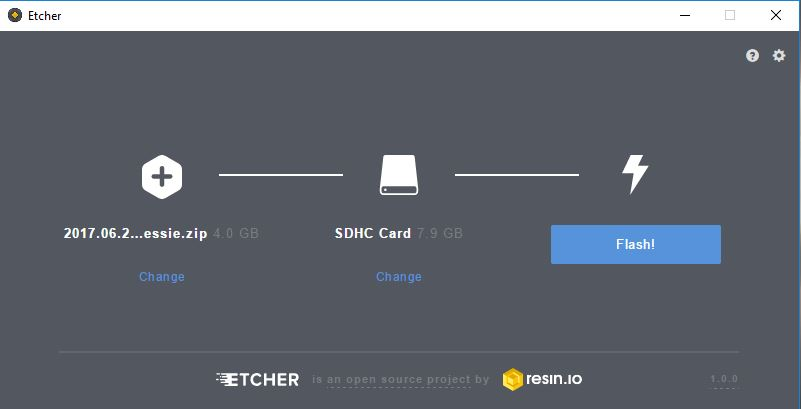
\includegraphics[width=.6\paperwidth]{images/etcher2.jpg}}
	\end{center}
		\caption{ \textit{Etcher prêt à flasher}}
	\end{figure}\\
\end{enumerate}
Et voilà, l'opération peut prendre une dizaine de minutes. C'était simple non ?

\section{Première mise en route de la \textit{RaspberryPi}.}

\begin{enumerate}

	\item Maintenant que vous avez \textit{Raspbian}, nous pouvons démarrer notre nouvel ordinateur.
Pour cela, il vous suffit d'insérer la microSD au dos de la \textit{RaspberryPi}.\\
\begin{figure}[H]
\begin{center}
	\makebox[\textwidth]{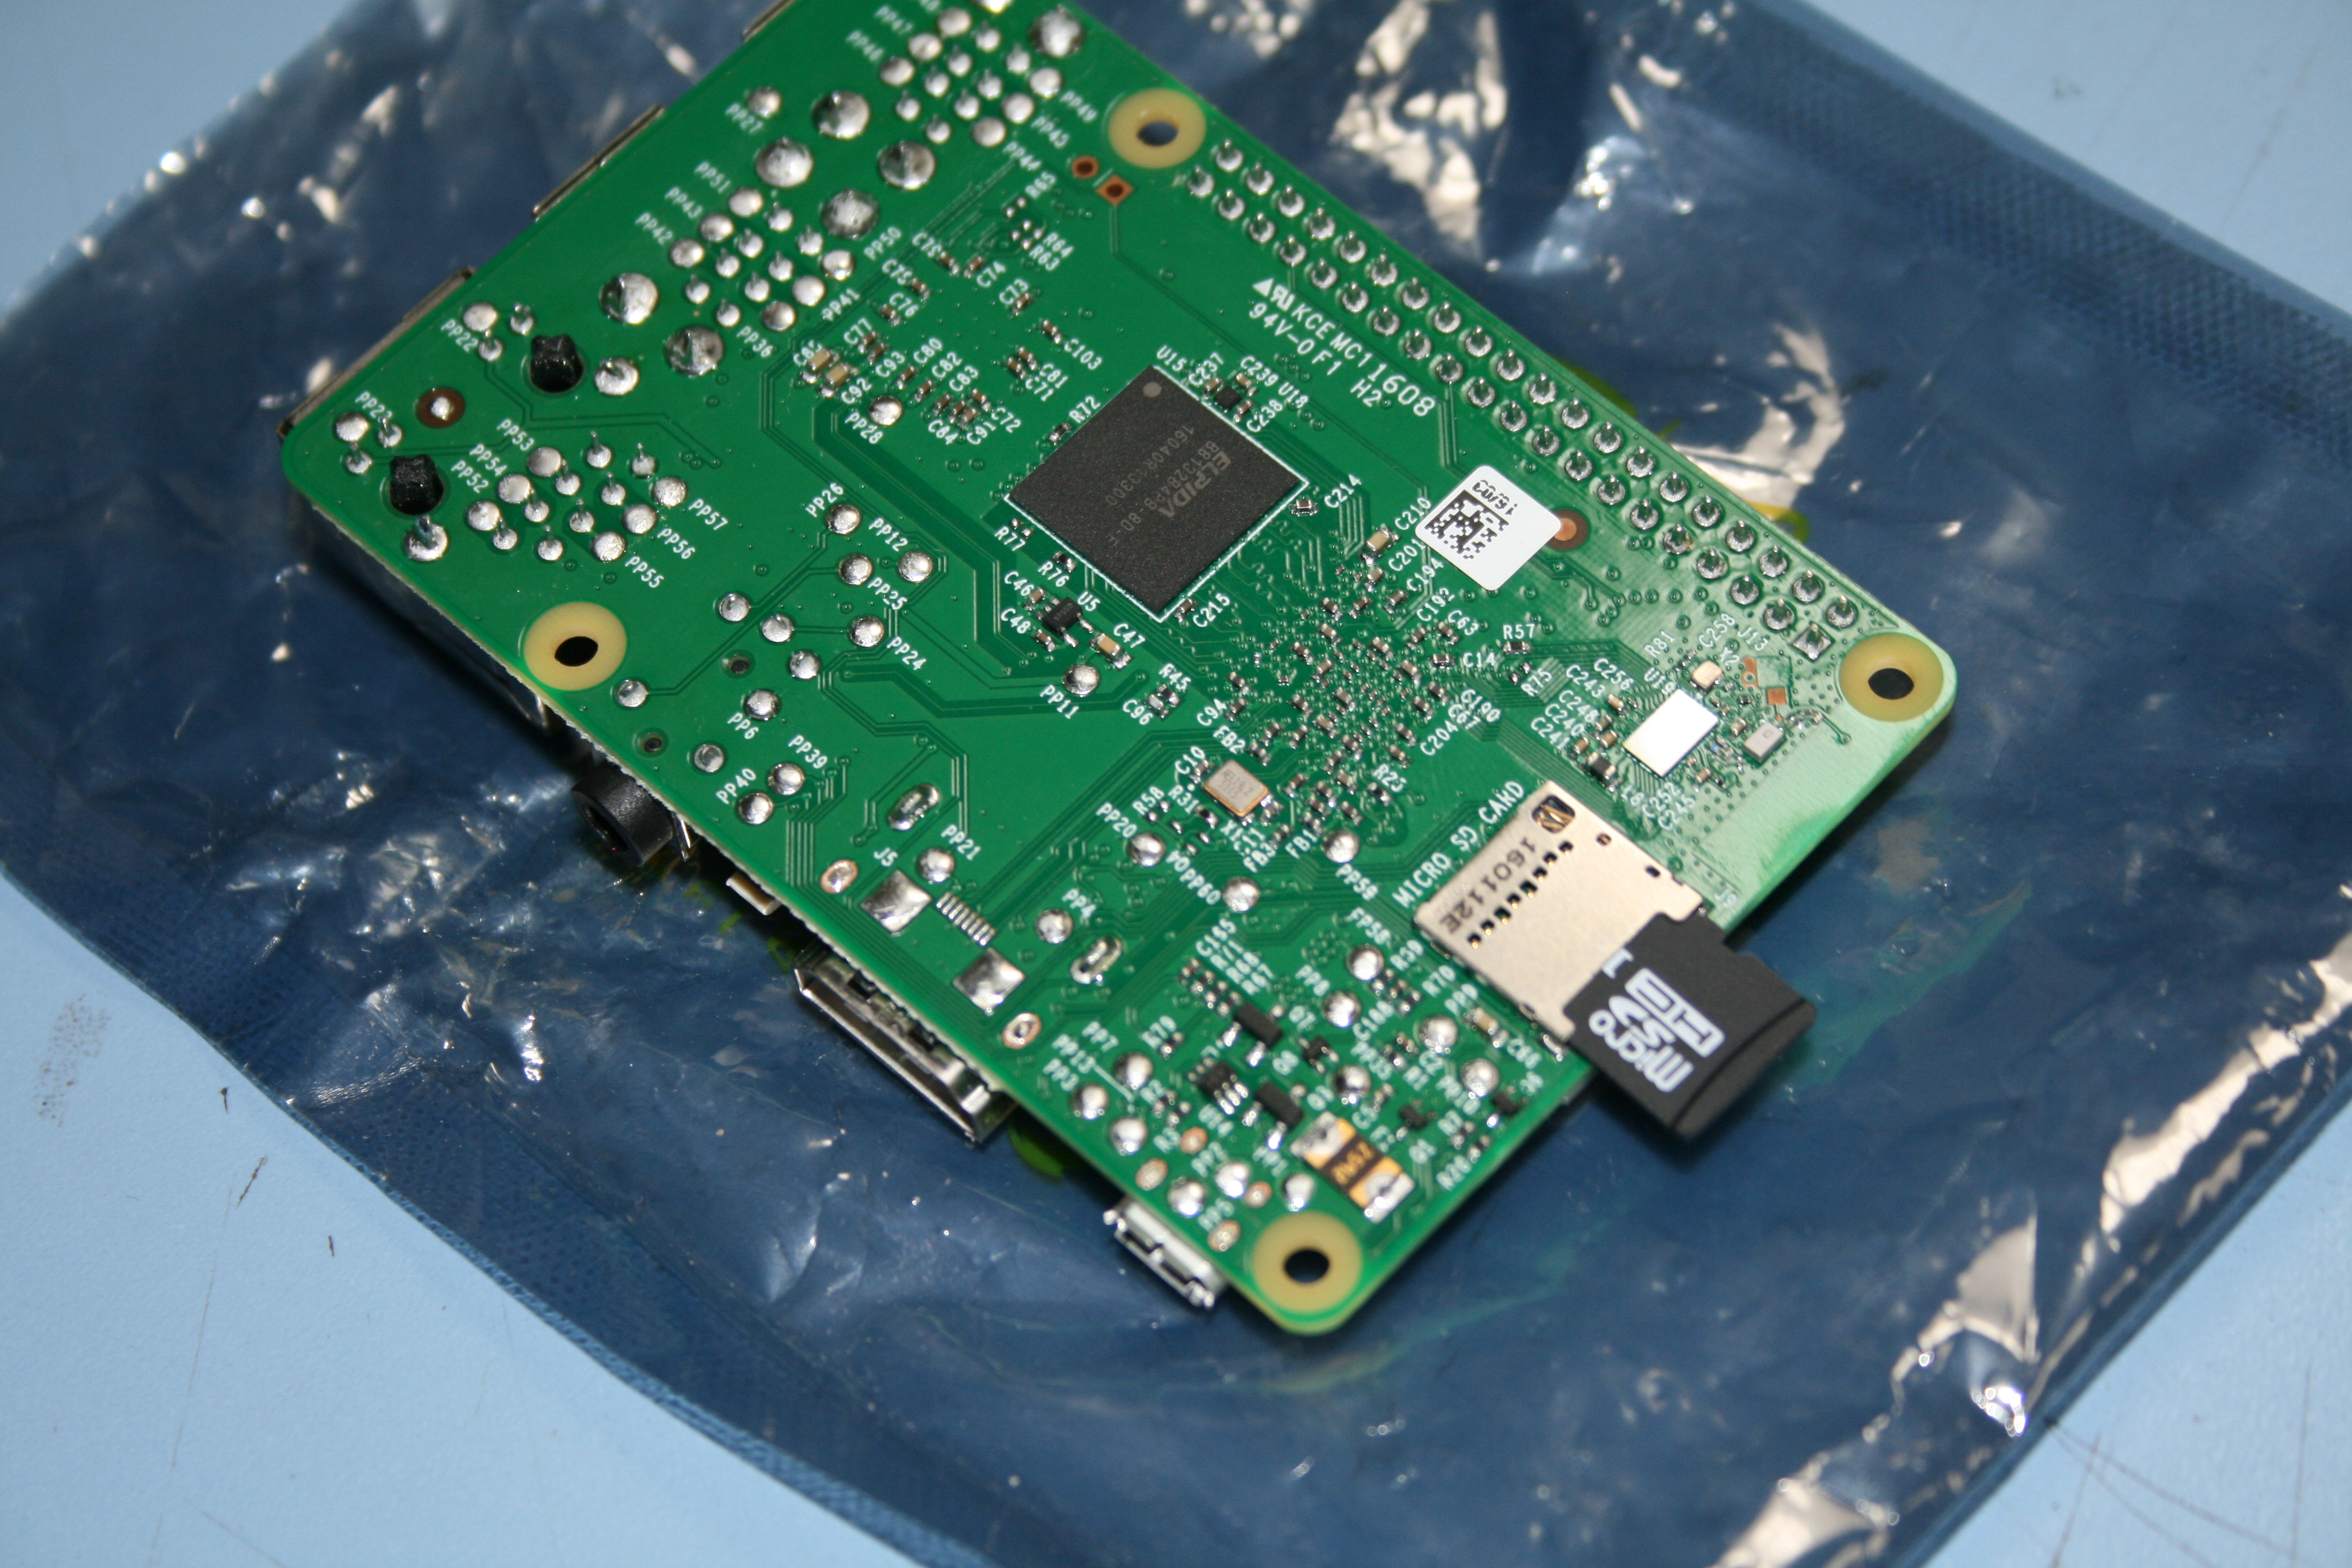
\includegraphics[width=.6\paperwidth]{images/microsd.jpg}}
\end{center}
	\caption{ \textit{La \textit{RaspberryPi} de dos}}
\end{figure}\\

	\item Ensuite, nous allons pouvoir lancer la \textit{RaspberryPi}. Avant de l'alimenter, nous allons distinguer deux cas.. Si vous avez la possibilité, de façon extérieur, d'accéder à l'adresse IP de votre \textit{RaspberryPi} alors vous pouvez sauter l'étape N°3. Si cela n'est pas possible, brancher un écran et un clavier.\\
	Vous pouvez maintenant l'alimenter en utilisant le port micro USB qui est à côté du port HDMI.\\
	
	\item Si vous suivez cette étape, vous devriez voir apparaître des lignes de commandes qui défilent. Quelques instants plus tard, vous arrivez sur l'environnement de bureau de votre \textit{RaspberryPi}.\\
	% faire la demarche pour ouvrir un terminal.
Une fois le terminal ouvert, entrer la commande suivante :\\
\begin{lstlisting}[style=MyBashStyle]
	sudo ifconfig
\end{lstlisting}
un mot de passe devrait vous être demandé, par défaut, le mot de passe est "robots1234"
%expliquer comment recuperer l'adresse IP et l'adresse MAC
	\item Très bien, désormais que vous avez l'adresse IP à disposition, nous allons pouvoir installer le nécessaire pour utiliser nos capteurs. Nous aurions très bien pu continuer cette installation directement sur la \textit{RaspberryPi} mais si vous n'avez jamais fait ce qui va suivre, cela vous fera un bon entrainement.\\

\begin{enumerate} 
	\item Télécharger et installer le logiciel \href{https://git-for-windows.github.io/}{Git Bash}. Ce logiciel permet l'utilisation d'un terminal plus avancé et compatible avec le langage système \textit{Bash}.
	\item Lancer \textit{Git Bash}
	\item taper la commande en remplaçant "xxx.xxx.xxx.xxx" par l'adresse IP de la \textit{RaspberryPi}\\
	\begin{lstlisting}[style=MyBashStyle]
	ssh pi@xxx.xxx.xxx.xxx
	\end{lstlisting}\\
la première fois, il vous sera demander si vous voulez réellement vous connecter sur le périphérique, taper alors "yes" puis sur la touche \textit{Entrée}
	\item Le mot de passe est "robots1234". Si tout c'est bien passé, vous devriez avoir cet aperçu :\\
	\begin{figure}[H]
	\begin{center}
		\makebox[\textwidth]{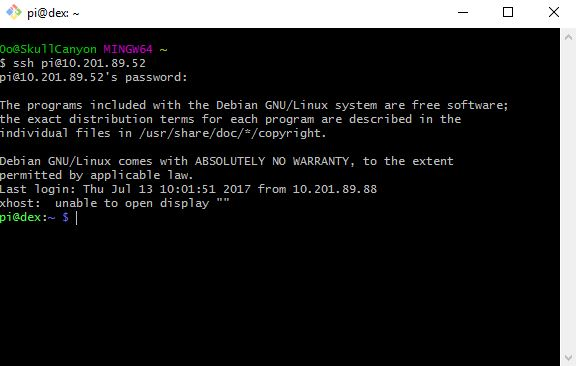
\includegraphics[width=.6\paperwidth]{images/ssh.jpg}}
	\end{center}
		\caption{ \textit{connexion à la RaspberryPi en SSH}}
	\end{figure}\\
	
	\item vous naviguez maintenant dans la \textit{RaspberryPi}. Dans un premier temps, nous allons changer le mot de passe car celui ci est un mot de passe par défaut. Enter la commande :\\
	\begin{lstlisting}[style=MyBashStyle]
	sudo raspi-config
	\end{lstlisting}\\
	un écran bleu devrait apparaître. %insérer image ici et expliquer le chmt mdp et expand
	
	\item Quitter le menu pour revenir au terminal. %expliciter
	\item Maintenant, nous allons installer GrovePi pour pouvoir utiliser le \textit{Shield}. Entrer alors les deux commandes suivantes :\\
	\begin{lstlisting}[style=MyBashStyle]
	sudo curl https://raw.githubusercontent.com/DexterInd
	/Raspbian_For_Robots/master/upd_script/fetch_grovepi.sh | bash
	 
	sudo reboot
	\end{lstlisting}\\
	Votre \textit{RaspberryPi} va redémarrer.
	\item Connecter vous à nouveau en "ssh" comme pour l'étape 4 mais cette fois ci avec votre nouveau mot de passe.
	\item Réaliser alors cette suite de commande une à une. Appuyer sur la touche \textit{Entrée} lorsque l'on vous demande de continuer :
	\begin{lstlisting}[style=MyBashStyle]
	cd /home/pi/Desktop
	sudo git clone https://github.com/DexterInd/GrovePi
	cd /home/pi/Desktop/GrovePi/Script
	sudo chmod +x install.sh
	sudo ./install.sh
	\end{lstlisting}\\
	
	\item Appuyez à nouveau sur \textit{Entrée} une fois arrivé sur cette configuration :
	%insérer image  
	\item Au moment où la \textit{RaspberryPi} va redémarrer (vous verrez un "Restart" écrit dans le terminal. Appuyez sur \textit{Ctrl + C} pour empêcher le redémarrage.
	\item Effectuer alors la commande :
	\begin{lstlisting}[style=MyBashStyle]
	sudo shutdown now
	\end{lstlisting}\\
	Elle va alors s'arrêter. Vous pouvez alors la débrancher après quelques instant.
	\end{enumerate}\\
	
		\item Vous pouvez désormais ajouter le \textit{Shield} sur la \textit{RaspberryPi} Comme ci-dessous \textbf{ATTENTION AU BROCHES UTILISÉES, BRANCHER LE SHIELD DANS LA MÊME CONFIGURATION QUE SUR LA PHOTO !}\\
		
	\begin{figure}[H]
	\begin{center}
		\makebox[\textwidth]{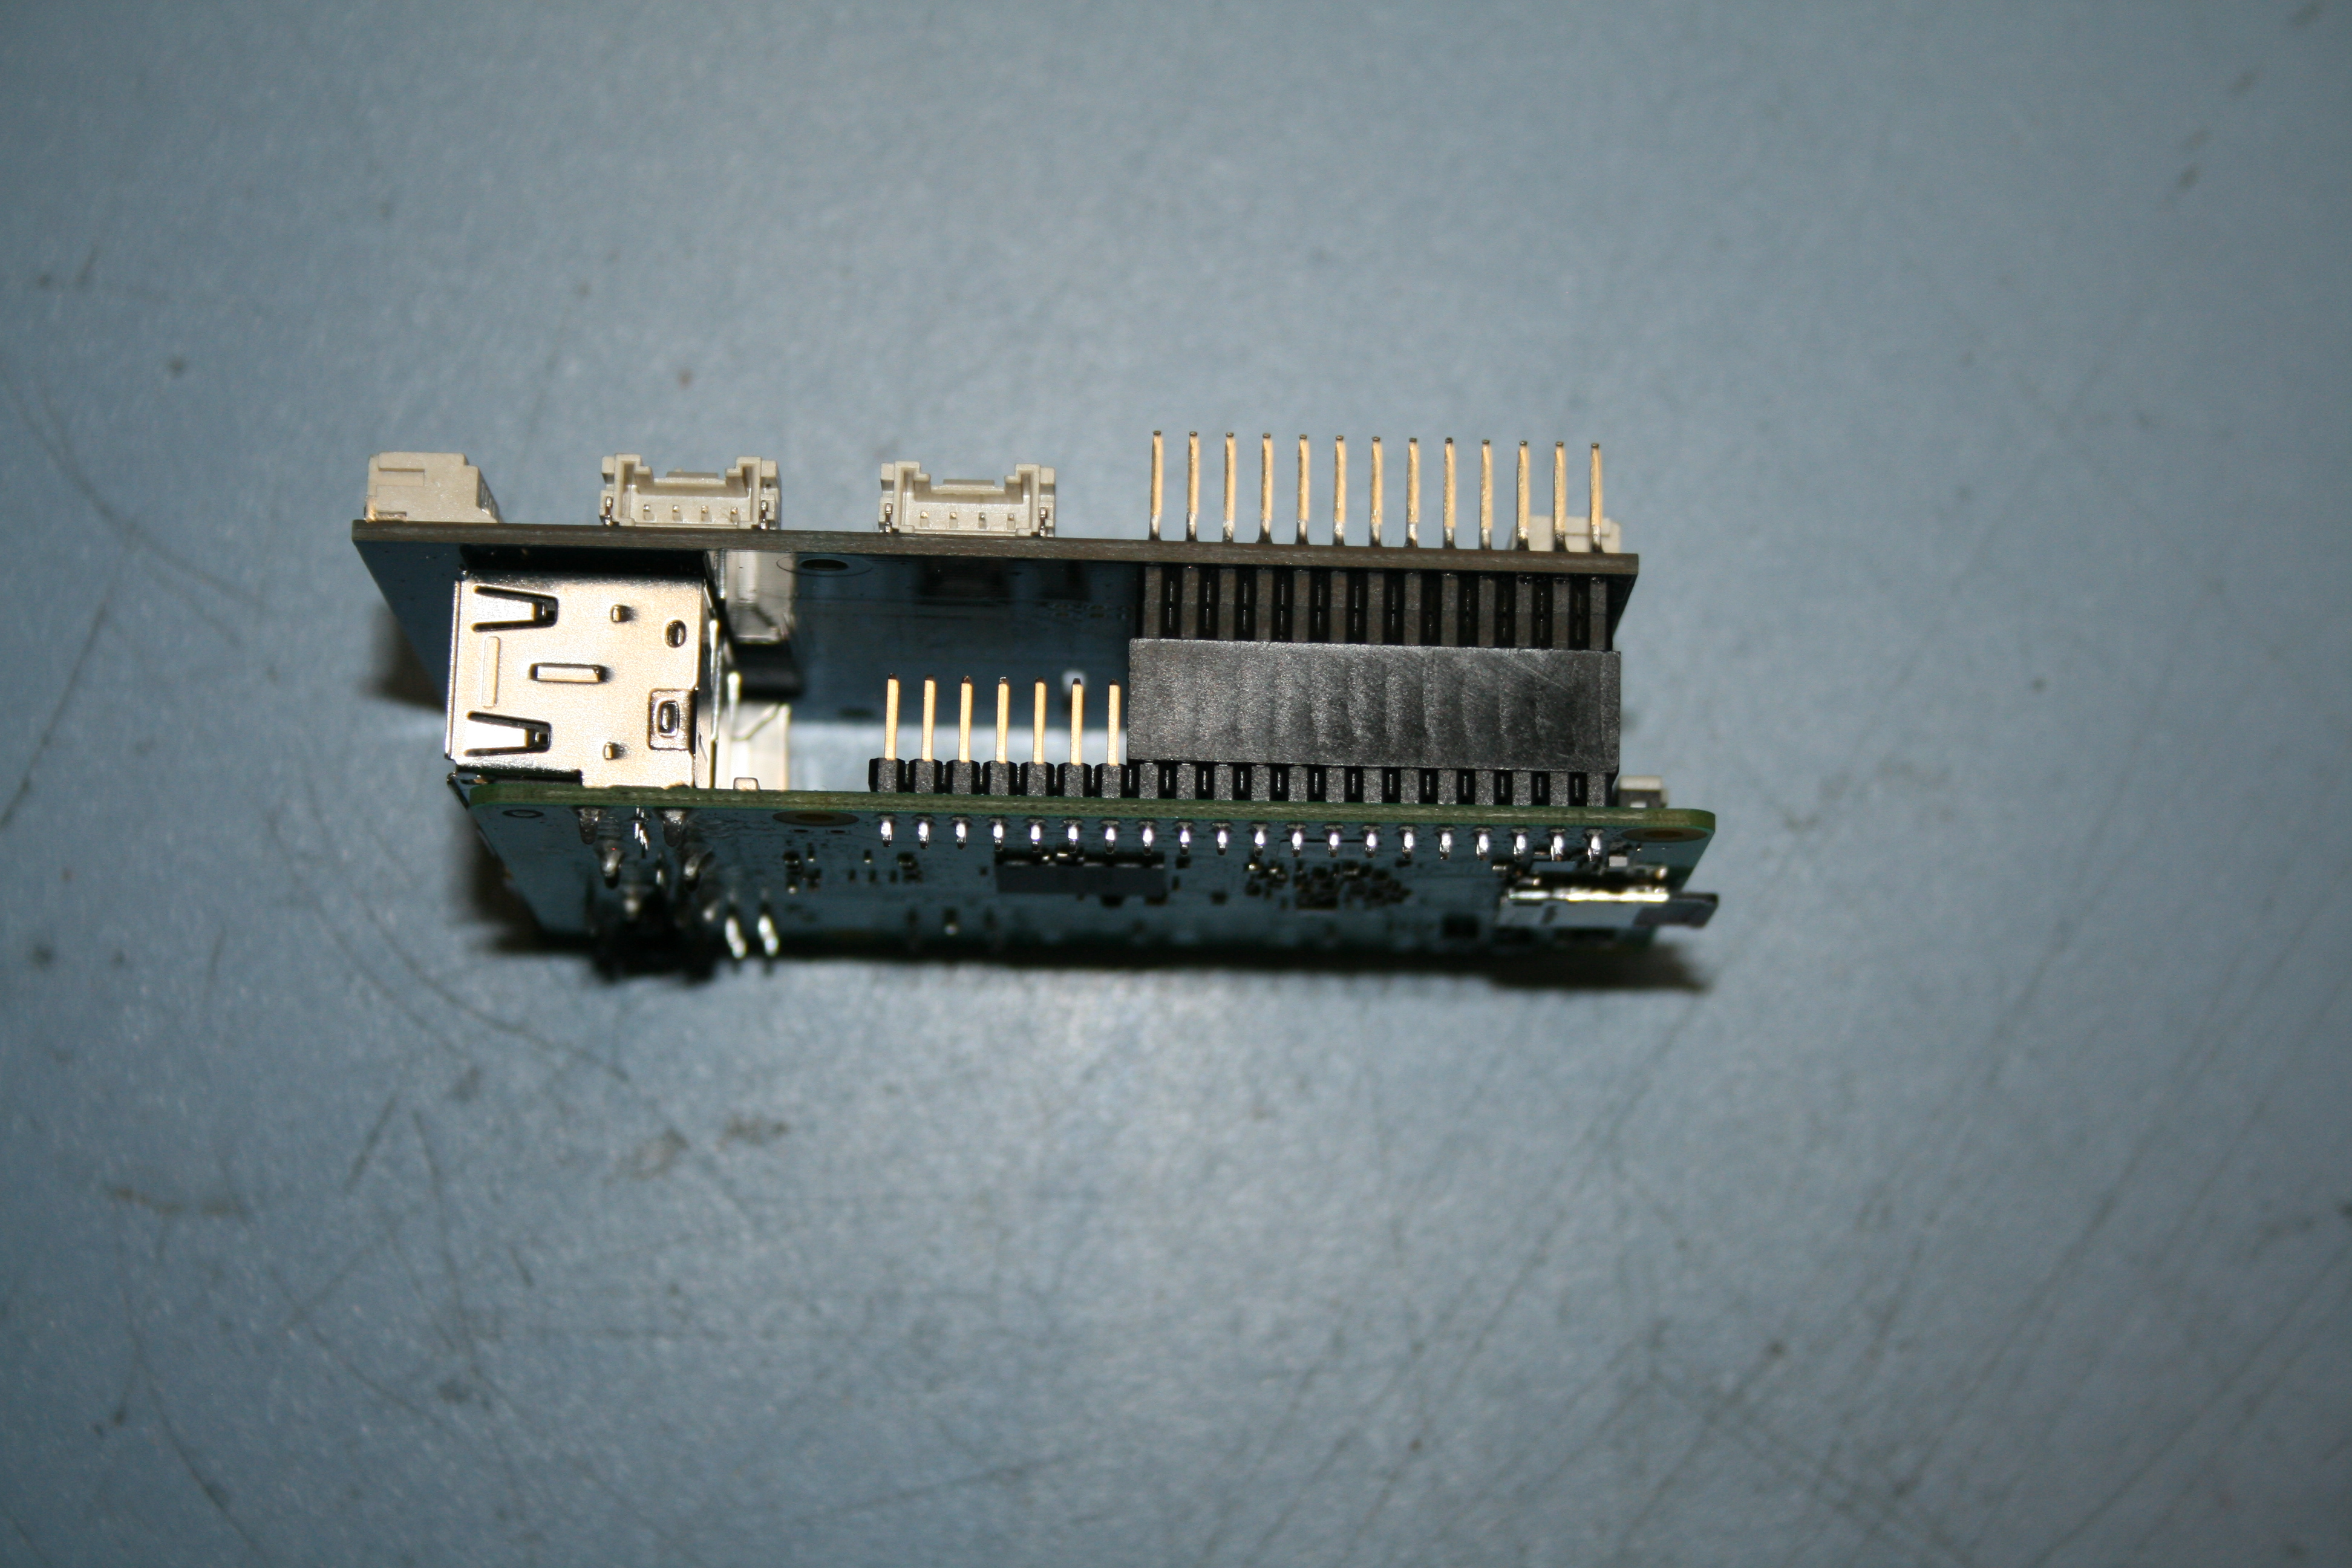
\includegraphics[width=.6\paperwidth]{images/branchement.jpg}}
	\end{center}
		\caption{ \textit{La RaspberryPi avec le Shield branché dessus}}
	\end{figure}\\
	
		\item Brancher à nouveau la \textit{RaspberryPi} au secteur. Vous devriez avoir une LED verte qui s'allume sur votre \textit{Shield}
		\item nous allons tester s'il a bien été reconnue, pour cela, connecter vous en "ssh" sur votre \textit{RaspberryPi} (vous devriez savoir le faire maintenant !)
		\item lancer la commande :
		\begin{lstlisting}[style=MyBashStyle]
		sudo i2cdetect -y 1
		\end{lstlisting}\\
	
vous devriez obtenir ce résultat, avec le 04 en première ligne. %ajouter image

\end{enumerate}\\

Voilà, la première mise en route de la \textit{RaspberryPi} est terminé, nous allons maintenant pouvoir nous occuper du code pour la station final.

\section{Installation, configuration et test du code de la station avec ses capteurs.}\\

\subsection{Installation des capteurs.}\\

Votre \textit{RaspberryPi} est configurée, ainsi que son \textit{Shield}. Nous allons maintenant pouvoir installer les différents capteurs. Regardons de plus près les différents connecteurs.\\

	\begin{figure}[H]
	\begin{center}
		\makebox[\textwidth]{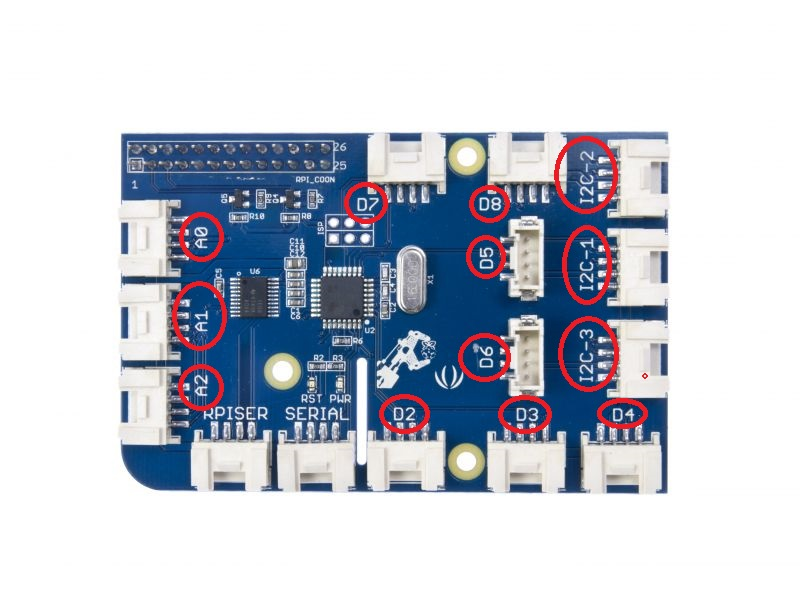
\includegraphics[width=.6\paperwidth]{images/grovepi_connecteur.jpg}}
	\end{center}
		\caption{ \textit{vu de dessus du shield}}
	\end{figure}\\
	
Comme vous pouvez le voir, il y a écrit un numéro d'identification du connecteur sur le \textit{Shield}. Vous allez donc brancher sur des ports particulier en adéquation avec le code qui sera télécharger ultérieurement.\\

Procéder aux branchement branchements suivants :
\begin{enumerate}
	\item Le capteur de température et d'humidité (DHT11) sur le port D7.
	\item Le capteur de luminosité sur le port A1.
	\item L'encodeur rotatif sur le port A2.
	\item L'écran LCD sur un des ports I2C.
\end{enumerate}
Vous devriez alors obtenir un résultat similaire à celui là :
	\begin{figure}[H]
	\begin{center}
		\makebox[\textwidth]{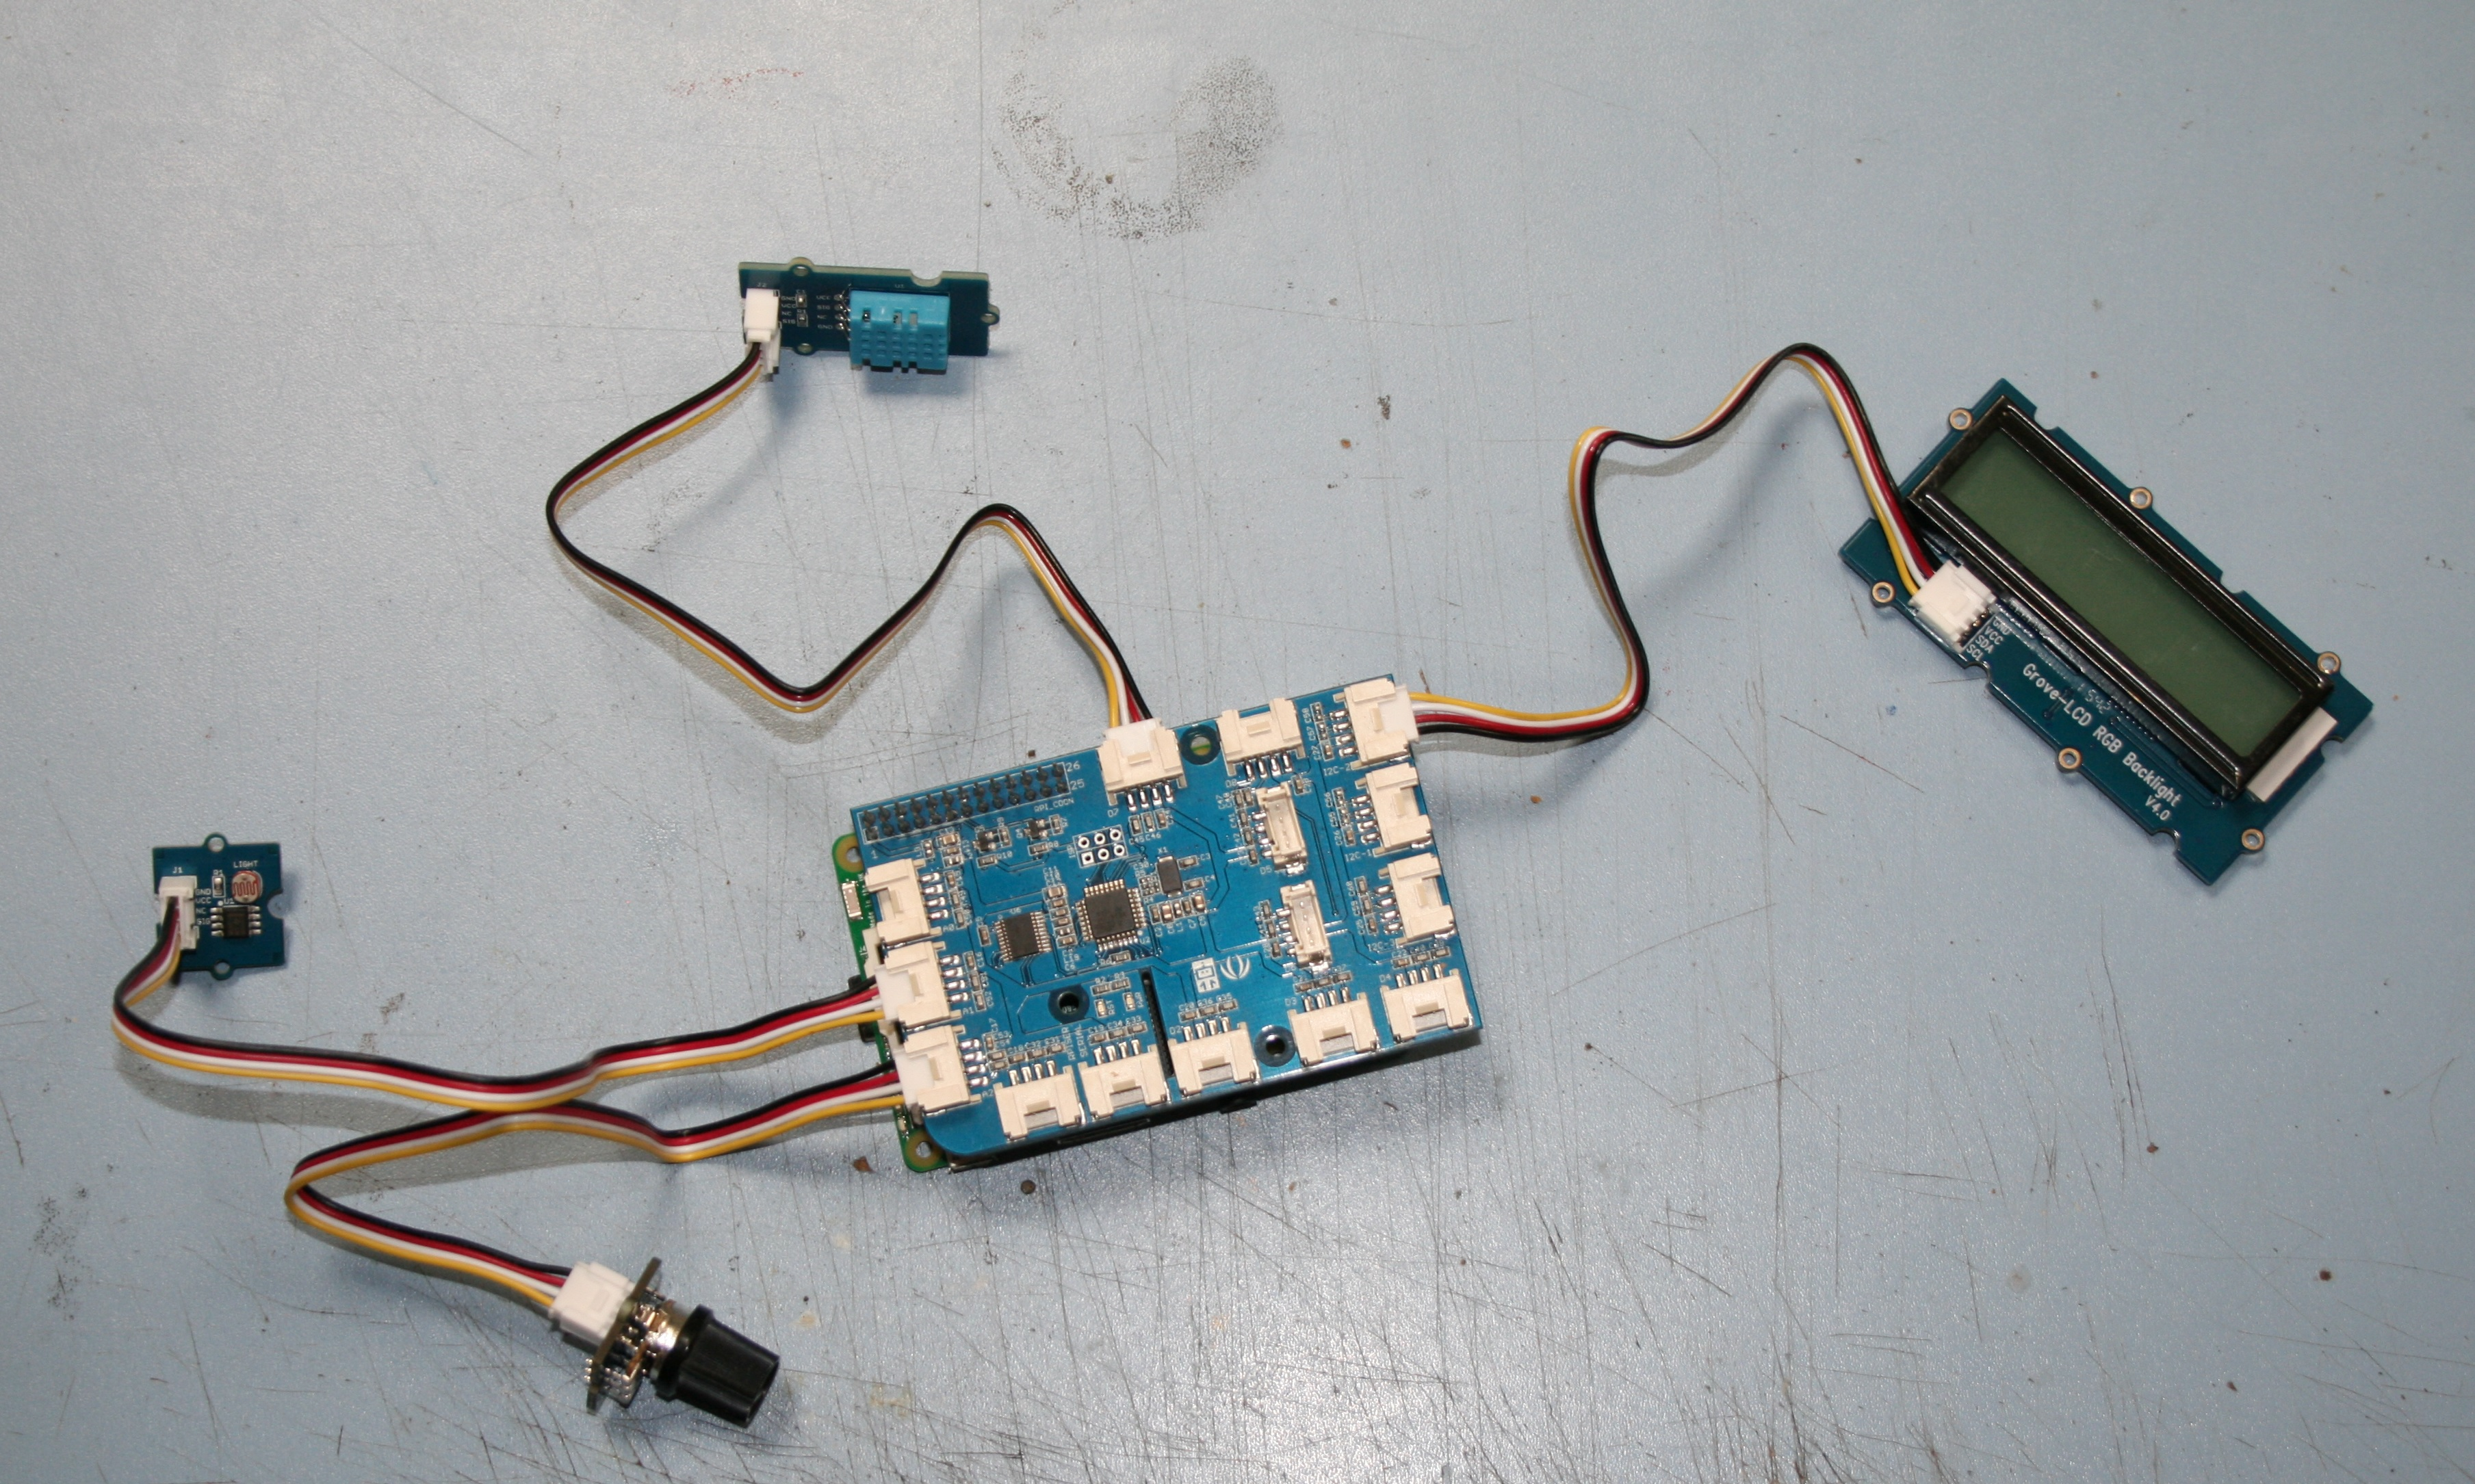
\includegraphics[width=.35\paperwidth]{images/branchement_final.jpg}} %photo a changer
	\end{center}
		\caption{ \textit{Branchement des compostant sur le shield}}
	\end{figure}\\

\subsection{Configuration de la \textit{RaspberryPi}.}\\

Nous allons maintenant télécharger le code pour activer le station. Pour cela, brancher votre \textit{RaspberryPi} au secteur et au réseau si jamais vous aviez enlevé le câble ethernet. Connectez vous en \textit{ssh} via \textit{git bash} et exécutez les deux commandes :\\
		\begin{lstlisting}[style=MyBashStyle]
	cd
	git clone https://github.com/Kymaro/stage_drancy
		\end{lstlisting}\\
%mettre la commande git clone du repo final

\\
Cette commande va télécharger le code nécessaire au fonctionnement de la station. Nous modifierons ce code dans le troisième chapitre pour envoyer les données sur le \textit{Cloud}.
\\

Tapez la commande :\\

\begin{lstlisting}[style=MyBashStyle]
	ls | grep stage_drancy
\end{lstlisting}\\%photo résultat

Si vous avez bien ce résultat, cela signifie que le code à bien été téléchargé et qu'il est présent dans le dossier \textit{stage_drancy} %mettre à jour le dossier nouveau repo
Si cela n'est pas le cas, réessayer la commande précédente.\\

Nous allons maintenant modifier un fichier dans \textit{Raspbian} pour faire en sorte que le script qui gère les capteurs puisse se lancer au démarrage de la \textit{RaspberryPi}.\\

Exécuter la commande : \\

\begin{lstlisting}[style=MyBashStyle]
	sudo nano /etc/rc.local
\end{lstlisting}\\

Un fichier va alors s'ouvrir dans votre terminal, vous ne pouvez pas utiliser la souris dans cet éditeur de texte. Descendez alors avec les flèches directionnelles jusqu'à l'avant dernière ligne, la dernière ligne étant normalement \textit{exit 0}. Allez à la fin de la ligne et appuyez alors sur \textit{Entrée} pour ajouter une nouvelle ligne. 
%commande rc local /home/pi/repogit/.../machin.py &
\\
Tapez alors sur cette nouvelle ligne :\\

\begin{lstlisting}[style=MyBashStyle]
	sudo python /home/pi/stage_drancy/rpi/test_complet.py &
\end{lstlisting}\\

L' esperluette permet d'exécuter le script en tâche de fond, il est important de ne pas l'oublier sinon votre \textit{RaspberryPi} ne sera pas capable de faire autre chose que de lancer votre script.

Pour quitter et enregistrer, taper sur la combinaison de touche une à une :\\

\begin{lstlisting}[style=MyBashStyle]
	Ctrl + X
	Y
	Entree
\end{lstlisting}\\

Nous sommes désormais prêt à tester la station.

\subsection{Test de la station}\\

Vous allez tout d'abord essayer la station en lançant le script manuellement pour vérifier que cela fonctionne, puis nous redémarrerons la \textit{RaspberryPi} pour voir si la modification de l'étape précédente est fonctionnelle.\\

Tapez la commande suivante pour lancer le script python (NOTE : Lorsque vous indiquez le chemin d'un fichier en \textit{Bash}, vous avez votre meilleur ami qui est là pour vous aider et qui s'appelle l'auto-complétion. En effet, lorsque vous commencer à écrire le nom d'un fichier, par exemple \textit{station_cloud}, il vous suffit d'écrire \textit{sta} puis d'appuyer sur la touche \textit{Tabulation} pour voir la suite se compléter. Si cela ne se complète pas, c'est que vous avez un autre fichier / dossier qui commence par \textit{sta}, vous devez alors écrire un caractère supplémentaire pour retenter votre chance ;) ) :\\

\begin{lstlisting}[style=MyBashStyle]
	cd
	sudo python stage_drancy/rpi/test_complet.py &
\end{lstlisting}\\

Cela ne vous rappelle rien ? Il s'agit ni plus ni moins de la ligne qui a été ajoutée dans le fichier \textit{/etc/rc.local} pour démarrer automatiquement le script. (il manque /home/pi/ puisque nous sommes dans ce dossier par défaut).

Vous devriez voir l'écran LCD de la station qui s'allume avec le message "Bienvenue dans l'IoT Hub" pendant quelques seconde puis un des menus qui affiche les données des capteurs. Si cela reste sur le premier message, tourner l'encodeur rotatif pour afficher les menus.

Si vous voyez bien tous les menus avec une valeur, on y est, la station fonctionne. Nous allons maintenant vérifier qu'elle démarre bien en même temps que la \textit{RaspberryPi}.
Mettons nous dans le scénario où elle a été coupé électriquement. 
Taper la commande :\\ %shutdown now.

\begin{lstlisting}[style=MyBashStyle]
	sudo shutdown now
\end{lstlisting}\\

Patienter quelques instants, débrancher puis rebrancher là. Vous devriez alors voir l'écran s'allumer comme pour le test précédent au bout d'un certain temps. %image.

Et voilà, nous arrivons au terme de ce chapitre, vous avez désormais une station fonctionnelle localement. Je vous invite alors à suivre le chapitre trois pour configurer \textit{Microsoft Azure} d'une part puis pour modifier le code de tel sorte qu'il envoie les messages sur \textit{le Cloud Azure}.



	
	
